\documentclass[11pt, a4paper]{article}
\usepackage{amsmath, amsthm, amssymb, bm, graphicx, hyperref, mathrsfs}
\usepackage[lined,boxed,commentsnumbered,linesnumbered,ruled]{algorithm2e}
\usepackage{enumitem}
% \title{\textbf{Difference Letter }}
% % \author{Dylaaan}
% \date{}
% \linespread{1.5}
\usepackage{longtable}
\usepackage{boxedminipage}
\usepackage{cite}
\usepackage{booktabs}
\usepackage{graphicx}
\usepackage{array}
\renewcommand{\baselinestretch}{1.15}
% \setlength{\parskip}{2mm}

\usepackage{graphicx}
\usepackage{caption}
\usepackage{subfig}
\usepackage{float}

\usepackage{booktabs}
\usepackage{epsfig,graphicx}

\newtheorem{definition}{Definition}
\newtheorem{theorem}{Theorem}
\newtheorem{lemma}{Lemma}
% \newtheorem{proof}{Proof}

\newtheorem{Example}{Example}

\setlength{\parskip}{1.5mm}
\setlength{\oddsidemargin}{0in}
\setlength{\evensidemargin}{1in}
\setlength{\topmargin}{0in}
\setlength{\headheight}{0in}
\setlength{\headsep}{0in}
\setlength{\textheight}{10in}
\setlength{\textwidth}{6.4in}

% \pagestyle{empty}


\begin{document}

\begin{center}
\Large{\textbf{Difference Letter}}\vspace{1mm}\\
\end{center}

\noindent
Dear Editor/Reviewer, 

We would like to submit the attached manuscript, ``A Spatio-Temporal Adaptive Framework for Dispatching, Routing, and Pricing of Bus-Booking'', for consideration for possible publication in your esteemed journal ``IEEE Transactions on Knowledge and Data Engineering  (TKDE)''.

The preliminary version of this paper, entitled ``SACA: An End-to-End Method for Dispatching, Routing, and Pricing of Online Bus-Booking'', was accepted by Database Systems for Advanced Applications (DASFAA 2023). There are significant differences between this journal submission and the conference version. We first highlight the main differences and then provide detailed descriptions following the organization of the manuscript. These differences are summarized as follows.

\noindent \textbf{Main differences}
\vspace{-1em}
\begin{itemize}
    \item[a)] \textbf{Problem Formulation Expansion:} We have significantly extended the original JDRP formulation in \textbf{Section III}. While the preliminary conference version mainly considered a stationary setting, this journal submission explicitly distinguishes between \textbf{Stationary JDRP (S-JDRP)} and \textbf{Robust JDRP (R-JDRP)} to better capture real-world demand volatility. We further model demand as stochastic and time-dependent, expand the notation system, and reformulate the objective as expected long-term profit under uncertainty.

    \item[b)] \textbf{From SACA to ST-SACA:} We extend the preliminary \textbf{SACA} framework into \textbf{ST-SACA} in \textbf{Section IV}. The major technical addition is a novel \textbf{Spatio-Temporal Adaptive Actor}, which integrates geographical coordinates and dynamic demand features via spatial self-attention. Compared with the original flat state representation, this new actor captures topological dependencies among stations and improves policy robustness under non-stationary demand.

    \item[c)] \textbf{Algorithmic and Theoretical Strengthening:} We add detailed training and online execution procedures in \textbf{Section IV-D}, together with a new theoretical analysis in \textbf{Section IV-E}. These additions analyze computational complexity, convergence guarantees, and robustness properties, thereby strengthening the reproducibility and enriching the theoretical foundation of the journal version.

    \item[d)] \textbf{Extensive Robustness-Oriented Experiments:} We substantially expand \textbf{Section V} by introducing non-stationary demand simulation, stronger baselines, training stability analysis, uncertainty-degree analysis, ablation studies, computational efficiency evaluation, and an enriched case study. These experiments demonstrate that ST-SACA improves both profit and robustness.

    \item[e)] \textbf{Expanded Motivation and Literature:} We reorganize the introduction and related work sections to more clearly describe the bus-booking service, explain the coupling among dispatching, routing, and pricing, and identify the research gap in spatio-temporal representation and robust learning. This revision provides a stronger conceptual foundation for the new ST-SACA design.
\end{itemize}

\newpage
 
\noindent \textbf{Detailed Descriptions of Differences}

\begin{itemize}
    \item[a)] In \textbf{Section I}, we substantially revised the Introduction to elevate the motivation from a bus-booking application description to a robustness-oriented problem narrative. The journal version now clarifies why bus-booking is important for Intelligent Transportation Systems, why the three operational decisions must be optimized jointly, and why a robust formulation is needed under non-stationary demand. The main textual differences are shown below.

    \textbf{Application motivation.} The conference version mainly introduced bus-booking as an efficient and economical public transportation service. The journal version further explains the spatio-temporal mismatch behind the service demand.

    \begin{tabular}{|p{0.44\textwidth}|p{0.44\textwidth}|}
        \hline
        \textbf{Original Version} & \textbf{New Version}\\
        \hline
        With the rapid expansion of urban scale and population growth, the demand for the timeliness and convenience of diversified urban transportation has been growing fast in recent years. However, existing transportation system is insufficient to meet the demand of passengers, especially for some transportation hubs at specific periods, such as airports at midnight, when the subways and buses are out of service~\cite{ref:odrp}. &
        With the rapid expansion of urban scales and population growth, traditional public transportation systems (e.g., subways and fixed-route buses) increasingly struggle to meet passengers' demands for timeliness and convenience. This issue is particularly acute due to the \textbf{spatio-temporal mismatch} between the operating windows of rigid transit schedules and the arrival patterns of passengers.\\
        \hline
    \end{tabular}

    \textbf{Problem scope and robustness.} The conference version formulated one JDRP problem under the basic online bus-booking setting. The journal version explicitly separates \textbf{Stationary JDRP (S-JDRP)} and \textbf{Robust JDRP (R-JDRP)}, which makes the gap between the preliminary setting and the more realistic non-stationary setting clear.

    \begin{tabular}{|p{0.44\textwidth}|p{0.44\textwidth}|}
        \hline
        \textbf{Original Version} & \textbf{New Version}\\
        \hline
        We first formulate the Joint order Dispatching, Route planning, and trajectory Pricing problem (JDRP), which is proven to be NP-hard. SACA determines the order price and the accepted order set according to the demand and supply relationship through a SAC framework, and then give the order dispatching and route planning solution with an attention mechanism, thus getting the new state of SAC. &
        To rigorously address these challenges, we formally define the \textbf{Joint order Dispatching, Route planning, and Trajectory Pricing (JDRP)} problem. We prove that JDRP is \textbf{NP-hard} via a reduction from the Traveling Salesman Problem (TSP). Beyond this inherent combinatorial complexity, the practical difficulty of the problem is further compounded by the specific assumptions regarding environmental dynamics: \textbf{The Stationary JDRP (S-JDRP)} assumes stationary demand patterns, while \textbf{The Robust JDRP (R-JDRP)} requires real-world platforms to cope with \textbf{dynamic uncertainty}, where demand intensity is non-stationary and governed by unknown distributions.\\
        \hline
    \end{tabular}

    \textbf{New contribution list.} The conference Introduction did not provide a separate contribution list. In the journal version, we add an explicit contribution summary to make the manuscript's extensions visible at the beginning of the paper.

    \begin{boxedminipage}[htbp]{\linewidth}
    \vspace{2mm}
    \noindent \textbf{New Version}
    \begin{itemize}
        \item \textbf{Problem Formulation and Analysis:} We systematically formulate the JDRP problem for bus-booking platforms and rigorously prove its NP-hardness via a reduction from the TSP. Crucially, we \textbf{explicitly distinguish} between the \textbf{Stationary JDRP} and the \textbf{Robust JDRP}, establishing a formalized bridge between theoretical simplifications and real-world volatility.
        \item \textbf{End-to-End Robust Framework:} We propose \textbf{ST-SACA}, an end-to-end framework that jointly optimizes dispatching, routing, and pricing. ST-SACA incorporates a novel \textbf{Spatio-Temporal Adaptive Actor}, which explicitly integrates geographical topology with demand features via self-attention, enabling the agent to learn resilient strategies against environmental uncertainty.
        \item \textbf{Realistic Mechanism Design:} We formulate the \textbf{economic interaction} between passengers and the platform by constructing distance-aware demand and supply functions. These designs capture not only the heterogeneous price sensitivity of passengers but also the supply willingness of the platform. Furthermore, we construct a multi-objective composite reward function that balances profit, order response rate, and operational costs to guide the policy toward long-term optimality.
        \item \textbf{Extensive Real-World Validation:} We conduct comprehensive experiments using a real-world trajectory dataset. The results demonstrate that our model outperforms state-of-the-art baselines, and exhibits superior robustness and performance stability under non-stationary environments.
    \end{itemize}
    \vspace{2mm}
    \end{boxedminipage}

    Overall, these revisions make the Introduction directly reflect the journal extension: the work is no longer presented only as an end-to-end solution for joint dispatching, routing, and pricing, but as a spatio-temporal adaptive framework for robust decision-making under real-world demand volatility.
    
    
    \item[b)] In \textbf{Section II}, we substantially revised the Related Work section so that it no longer serves only as a general survey of dispatching, routing, and pricing methods. In the journal version, Section II is reorganized as a gap-driven discussion that directly motivates the three major extensions of this submission: end-to-end joint optimization with pricing, trajectory-aware economic modeling, and spatio-temporal robust learning.

    \textbf{From component-wise background to joint-optimization gap.} The conference version reviewed order dispatching, route planning, and trajectory pricing mostly as separate technical topics, and concluded with the absence of an end-to-end solution for the three tasks. The journal version sharpens this argument by explaining why existing methods remain insufficient even when two tasks are jointly considered: they still miss the economic lever of pricing and the resulting routing-cost feedback.
    
    \begin{tabular}{|p{0.44\textwidth}|p{0.44\textwidth}|}
        \hline
        \textbf{Original Version} & \textbf{New Version}\\
        \hline
        In recent years, order dispatching is usually considered jointly when solving route planning or trajectory pricing problems. Machine learning methods were proposed to solve the joint problems of the two issues. However, there exists no learning-based approach to solve the joint problem of the three issues in an end-to-end manner. Compared with the multi-stage methods for the joint problem, our proposed end-to-end framework is able to explore more feasible spaces to discover globally better solutions. &
        Despite these advancements, most existing studies treat dispatching and routing as sequential, independent tasks~\cite{ref:DPEA} or focus on specific sub-problems like demand-aware routing~\cite{ref:DemandAware}. Few frameworks achieve a truly end-to-end joint optimization of dispatching and routing while simultaneously considering the economic lever of pricing. Neglecting this coupling often leads to suboptimal solutions where accepted orders may incur excessive routing costs.\\
        \hline
    \end{tabular}

    \textbf{From general dynamic pricing to trajectory-aware pricing.} The conference version mainly explained why SAC is suitable for continuous pricing. The journal version further identifies a more specific limitation of existing pricing studies: they usually ignore the spatial heterogeneity of destinations and the routing burden imposed by each accepted order. This revision directly motivates the distance-aware demand-supply mechanism introduced later in the manuscript.
    
    \begin{tabular}{|p{0.44\textwidth}|p{0.44\textwidth}|}
        \hline
        \textbf{Original Version} & \textbf{New Version}\\
        \hline
        However, these RL-based methods are not suitable for bus-booking pricing since Q-learning framework is designed for discrete action space. We therefore apply the SAC network to the continuous action (pricing) space and design novel demand and supply functions. &
        To capture long-term dependencies, RL-based pricing strategies have been introduced~\cite{ref:Lei2023, ref:Ge2025}. A challenge is the continuous nature of price values. The standard Q-learning methods designed for discrete action spaces are not suitable for fine-grained pricing. While recent works attempted to handle continuous action spaces~\cite{ref:ROSDR}, they typically assume a homogeneous relationship between demand and price across different destinations.\\
        \hline
        Dynamic pricing was the main strategy for the trajectory pricing problem in the early days~\cite{ref:PODP}. However, it usually does not take into account long-term revenue because it is highly susceptible to short-term fluctuations in supply and demand. &
        In the context of bus-booking, pricing must be \textit{trajectory-aware}. Existing methods often overlook the spatial heterogeneity of operational costs. Orders with different destinations impose vastly different routing burdens on the bus. Our work addresses this by integrating a distance-aware demand-supply function within a continuous control RL framework.\\
        \hline
    \end{tabular}

    \textbf{New review perspective on spatio-temporal robustness.} The conference version did not discuss spatio-temporal representation or robustness as a separate research gap. The journal version adds a dedicated subsection, \textbf{Spatio-Temporal Representation and Robust Learning}, to explain why a flat state representation and stationary-environment assumption are insufficient for real-world bus-booking platforms.

    \begin{boxedminipage}[htbp]{\linewidth}
    \vspace{2mm}
    \noindent \textbf{New Version}
    
    Effective decision-making in transportation requires capturing complex spatio-temporal dependencies. While early works relied on statistical models like ARIMA, deep learning approaches such as Graph Neural Networks (GNNs) and Attention mechanisms have become the state-of-the-art for modeling traffic flows~\cite{ref:STPivotal} and spatial correlations~\cite{ijcai/YuYZ18}. However, standard RL architectures used in dispatching often treat the system state as a flat feature vector, neglecting the underlying topological structure of the station network.

    Furthermore, real-world operations are plagued by dynamic uncertainty. Standard RL assumes a stationary environment, leading to performance degradation when deployed in non-stationary real-world scenarios. Robust RL aims to learn policies resilient to environmental parameter variations~\cite{ref:RobustRoute, ref:RobustMARL} or out-of-distribution scenarios~\cite{ref:Yoon2024IJCAI}.

    Although our preliminary work, SACA~\cite{ref:saca}, proposed a joint optimization framework, it relied on stationary environmental assumptions. There is a lack of unified frameworks that explicitly model the topological dependencies of station networks while ensuring robustness against non-stationary demand. Our proposed ST-SACA fills this void by introducing a Spatio-Temporal Adaptive Actor within a maximum entropy RL framework to cope with the non-stationary demand.
    \vspace{2mm}
    \end{boxedminipage}

    Overall, the revised Related Work section now plays a stronger argumentative role. It connects prior studies to the specific limitations addressed in this journal version and prepares the reader for the later distinction between \textbf{S-JDRP} and \textbf{R-JDRP}, the distance-aware pricing mechanism, and the \textbf{Spatio-Temporal Adaptive Actor}.

    \item[c)] In \textbf{Section III}, we substantially expanded the original problem statement into a more complete modeling section. The conference version mainly introduced the basic entities and defined one JDRP problem. The journal version turns this section into the formal foundation of the whole manuscript by adding a notation table, introducing the station network and stochastic demand, rewriting the objective under uncertainty, distinguishing \textbf{S-JDRP} and \textbf{R-JDRP}, and adding a case study to illustrate the coupled decisions.

    \textbf{Expanded notation system and preliminary entities.} The conference version defined entities directly in the text. The journal version adds a dedicated notation table and revises the entity definitions so that the formulation can support station topology, time-dependent orders, dynamic bus availability, stochastic demand, and policy-based decision making.

    \begin{tabular}{|p{0.44\textwidth}|p{0.44\textwidth}|}
        \hline
        \textbf{Original Version} & \textbf{New Version}\\
        \hline
        To cope with online scenarios of the bus-booking service, we adopt the round-based model. In each round, the platform operates on pended orders and available buses to optimize some objectives. Some basic features are introduced here. &
        In this section, we formally formulate the \textit{Joint order Dispatching, Route planning, and trajectory Pricing} (JDRP) problem. We first introduce the foundational entities and the general problem formulation. Subsequently, we discuss two variants of the JDRP problem: the \textit{Stationary JDRP} (S-JDRP)~\cite{ref:odrp} problem under stationary demand, and the \textit{Robust JDRP} (R-JDRP) problem under dynamic uncertainty.\\
        \hline
    \end{tabular}

    \begin{boxedminipage}[htbp]{\linewidth}
    \vspace{2mm}
    \noindent \textbf{New Version: Key Notation Categories}
    
    The journal version adds a notation table, which summarizes the symbols by categories, including \textbf{Sets \& Graph} ($G$, $loc_k$, $\mathcal{B}$, $\mathcal{B}^t$, $\mathcal{O}^t$), \textbf{Uncertainty} ($\mathcal{P}(\lambda^t)$, $\lambda^t$), \textbf{Order Entity} ($o_j$, $d_j$, $c^o_j$), \textbf{Bus Entity} ($b_i$, $r_i^t$, $L_i$, $c^b_i$, $v_i$), \textbf{Calculation} ($T$, $\text{cost}_i$, $dis_i$, $\beta_d$, $p_j$), and \textbf{Decision \& Obj.} ($x_{ij}^t$, $\pi$, $R^t$, $\mathbb{E}[\sum R^t]$).
    \vspace{2mm}
    \end{boxedminipage}

    \textbf{From deterministic entities to stochastic and topological modeling.} The conference version described orders and buses in a compact deterministic form. The journal version adds an explicit \textbf{Station Network} definition and rewrites the demand model as an unknown time-dependent stochastic process, which is essential for the later robust formulation.

    \begin{tabular}{|p{0.44\textwidth}|p{0.44\textwidth}|}
        \hline
        \textbf{Original Version} & \textbf{New Version}\\
        \hline
        The passenger demand $D_k^t$ in the time slot $t$ is represented by the number of passengers whose destination is $d_k$. &
        In real-world scenarios, passenger demand is stochastic and fluctuates over time. We model the underlying demand potential at station $k$ during time slot $t$ as a variable governed by a time-dependent probability distribution $\mathcal{P}(\lambda^t_k)$, where $\lambda^t_k$ represents the varying demand intensity. Crucially, this distribution is \textbf{unknown} to the platform.\\
        \hline
    \end{tabular}

    \begin{boxedminipage}[htbp]{\linewidth}
    \vspace{2mm}
    \noindent \textbf{New Version: Station Network}
    
    The city station network is modeled as a graph $G=(V, E)$, where $V$ represents the set of stations (including the departure station $DS$ and all potential destinations), and $E$ represents the connectivity (road paths) between stations. Each station $v_k \in V$ is associated with a static coordinate $loc_k = (x_k, y_k)$. This spatial information defines the underlying topology of the network, which determines the travel distance between stations.
    \end{boxedminipage}

    \textbf{Reformulated objective under uncertainty.} The conference version defined JDRP as maximizing long-term revenue. The journal version rewrites the objective as expected long-term profit over stochastic order arrivals, explicitly incorporates operating cost, and represents the platform decision as a policy that jointly outputs pricing, assignment, and routing decisions.

    \begin{tabular}{|p{0.44\textwidth}|p{0.44\textwidth}|}
        \hline
        \textbf{Original Version} & \textbf{New Version}\\
        \hline
        Given inputs of departure station $DS$, order set $O$ and bus set $B$, the JDRP problem for the bus-booking platform is to determine prices, dispatch orders to buses and plan bus routes such that the long-term revenue $R^{all}$ is maximized, while satisfying four constraints mentioned above. &
        Given the station network $G$ and the bus fleet $\mathcal{B}$, consider an environment where the passenger demand is governed by an unknown stochastic process. \textbf{Joint order Dispatching, Route planning, and trajectory Pricing (JDRP)} problem aims to learn a policy $\pi$ that generates the decision tuple $\langle \mathbf{Price}^t, \mathbf{X}^t, \mathbf{Route}^t \rangle$ for $\mathcal{O}^t$, $\mathcal{B}^t$ to maximize the \textbf{expected} long-term profit over the horizon $T$, subject to the above constraints.\\
        \hline
    \end{tabular}

    \begin{boxedminipage}[htbp]{\linewidth}
    \vspace{2mm}
    \noindent \textbf{New Version: Profit and Expected Objective}
    \begin{equation}
        R^t = \sum_{o_j \in \mathcal{O}^t} \left( p_j \cdot \sum_{b_i \in \mathcal{B}^t} x_{ij}^t \right) - \sum_{b_i \in \mathcal{B}^t} \text{cost}_i,
    \end{equation}
    where $\text{cost}_i = \beta_d \cdot dis_i$ is the operational cost for bus $b_i$.
    \begin{equation}
        \max_{\pi} \sum_{t=1}^T \mathbb{E}_{\mathcal{O}^t \sim \mathcal{P}(\lambda^t)}\left[R^t\right].
    \end{equation}
    \vspace{1mm}
    \end{boxedminipage}

    \textbf{Formal distinction between S-JDRP and R-JDRP.} The conference version implicitly worked under a stable environment. The journal version explicitly separates the stationary setting from the robust non-stationary setting, which clarifies the theoretical scope of the preliminary work and motivates the new robust framework.

    \begin{tabular}{|p{0.44\textwidth}|p{0.44\textwidth}|}
        \hline
        \textbf{Original Version} & \textbf{New Version}\\
        \hline
        The conference version formulated one JDRP problem and did not distinguish different stationarity assumptions of passenger demand. &
        \textbf{1) The Stationary JDRP (S-JDRP):} This variant operates under the assumption that the demand distribution is \textbf{stationary} over time. In this setting, demand patterns are stable or strictly cyclic. This formulation aligns with the assumptions made in our preliminary work~\cite{ref:odrp} and most traditional multi-stage approaches.

        \textbf{2) The Robust JDRP under Non-Stationarity (R-JDRP):} This variant relaxes the stationarity assumption to model realistic urban dynamics. Here, the demand intensity is governed by a \textbf{non-stationary} stochastic process with unknown distributional shifts. This represents a generalized and more challenging form of the problem, requiring algorithms with strong adaptability and robustness.\\
        \hline
    \end{tabular}

    \textbf{Added case study and updated hardness analysis.} The journal version adds a toy example to make the coupled effect of pricing, dispatching, routing, and bus reservation visible before the algorithmic section. The NP-hardness discussion is also rewritten in a concise proof form based on a reduction from TSP.

    \begin{boxedminipage}[htbp]{\linewidth}
        \vspace{2mm}

        \noindent \textbf{New Version: Case Study}

        \begin{center}
            \makeatletter
            \def\@captype{figure}
            \makeatother
            
            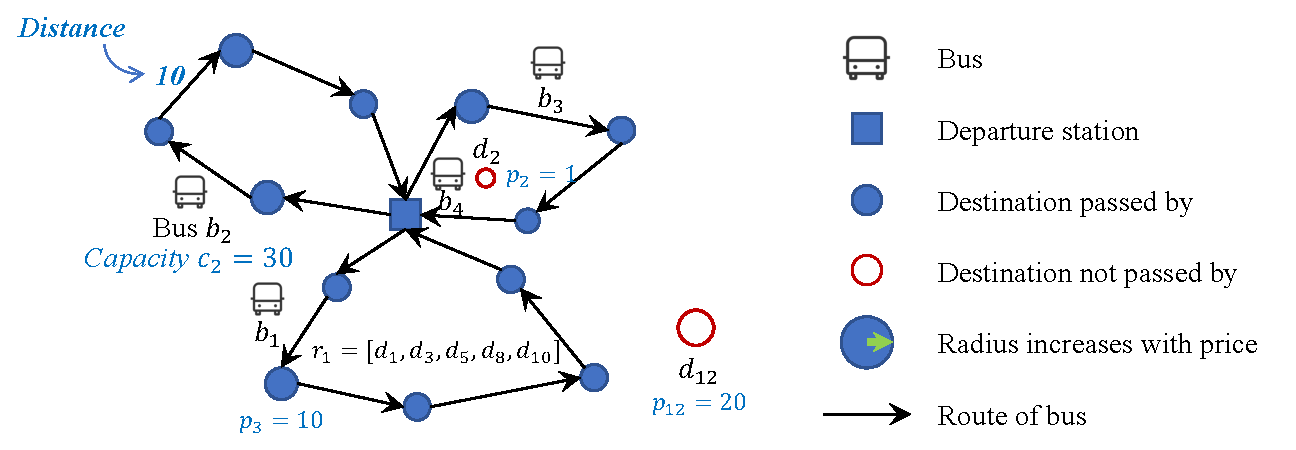
\includegraphics[width=0.5\linewidth]{fig/toyexample.pdf}
            \caption{Toy example added in the journal version.} 
            \label{fig:reply_toyexample}
        \end{center}
    \end{boxedminipage}

    \begin{boxedminipage}[htbp]{\linewidth}
        \vspace{2mm}

        A toy example of a single time slot for the JDRP problem is shown in Figure~\ref{fig:reply_toyexample}, where the solid point represents the departure station $DS$, each point represents the destination of the passenger, and edges represent planned routes. In the toy example, four buses depart from the same departure station $DS$, while some orders with different destinations are submitted to the platform. Under constraints mentioned above, the platform decides which orders to accept, determines their prices, and plans routes for buses to maximize the profit, while may reserve some buses for use in the next time slot, such as $b_4$. $d_2$ and $d_{12}$ denoted by red hollow points are rejected. Specifically, though $d_2$ is close to $DS$ which implying the cost for platform to passing by $d_2$ is low, a low price of orders to $d_2$ results in rejection. $d_{12}$ is not passed by because $d_{12}$ is far from $DS$. Besides, the route of $b_1$ consists of destinations of the orders assigned to the bus, i.e., $r_1 = [d_1, d_3, d_5, d_8, d_{10}]$.
    \end{boxedminipage}

    Overall, Section III now provides a substantially stronger foundation for the journal version: it makes the notation reproducible, exposes the station topology and demand uncertainty, formalizes the robust problem variant, and explains the operational coupling through an explicit example.

    \item[d)] In \textbf{Section IV}, we substantially expanded the method section from the preliminary \textbf{SACA} pipeline into the new \textbf{ST-SACA} framework. The conference version mainly combined SAC-based pricing with attention-based routing. The journal version further introduces a robustness-oriented architecture, including distance-aware demand-supply interaction modeling, a \textbf{Spatio-Temporal Adaptive Actor}, explicit training and online execution workflows, and a new theoretical analysis of real-time feasibility and robustness.

    \textbf{From a two-module pipeline to a robustness-oriented framework.} The journal version redraws the overall framework to clarify how market interaction, robust pricing/dispatching, and routing are connected. This makes the data flow among demand response, seat allocation, route generation, and reward feedback much more explicit than in the conference version.

    \begin{boxedminipage}[htbp]{\linewidth}
        \vspace{2mm}

        \noindent \textbf{New Version}

        \begin{center}
            \makeatletter
            \def\@captype{figure}
            \makeatother
            
            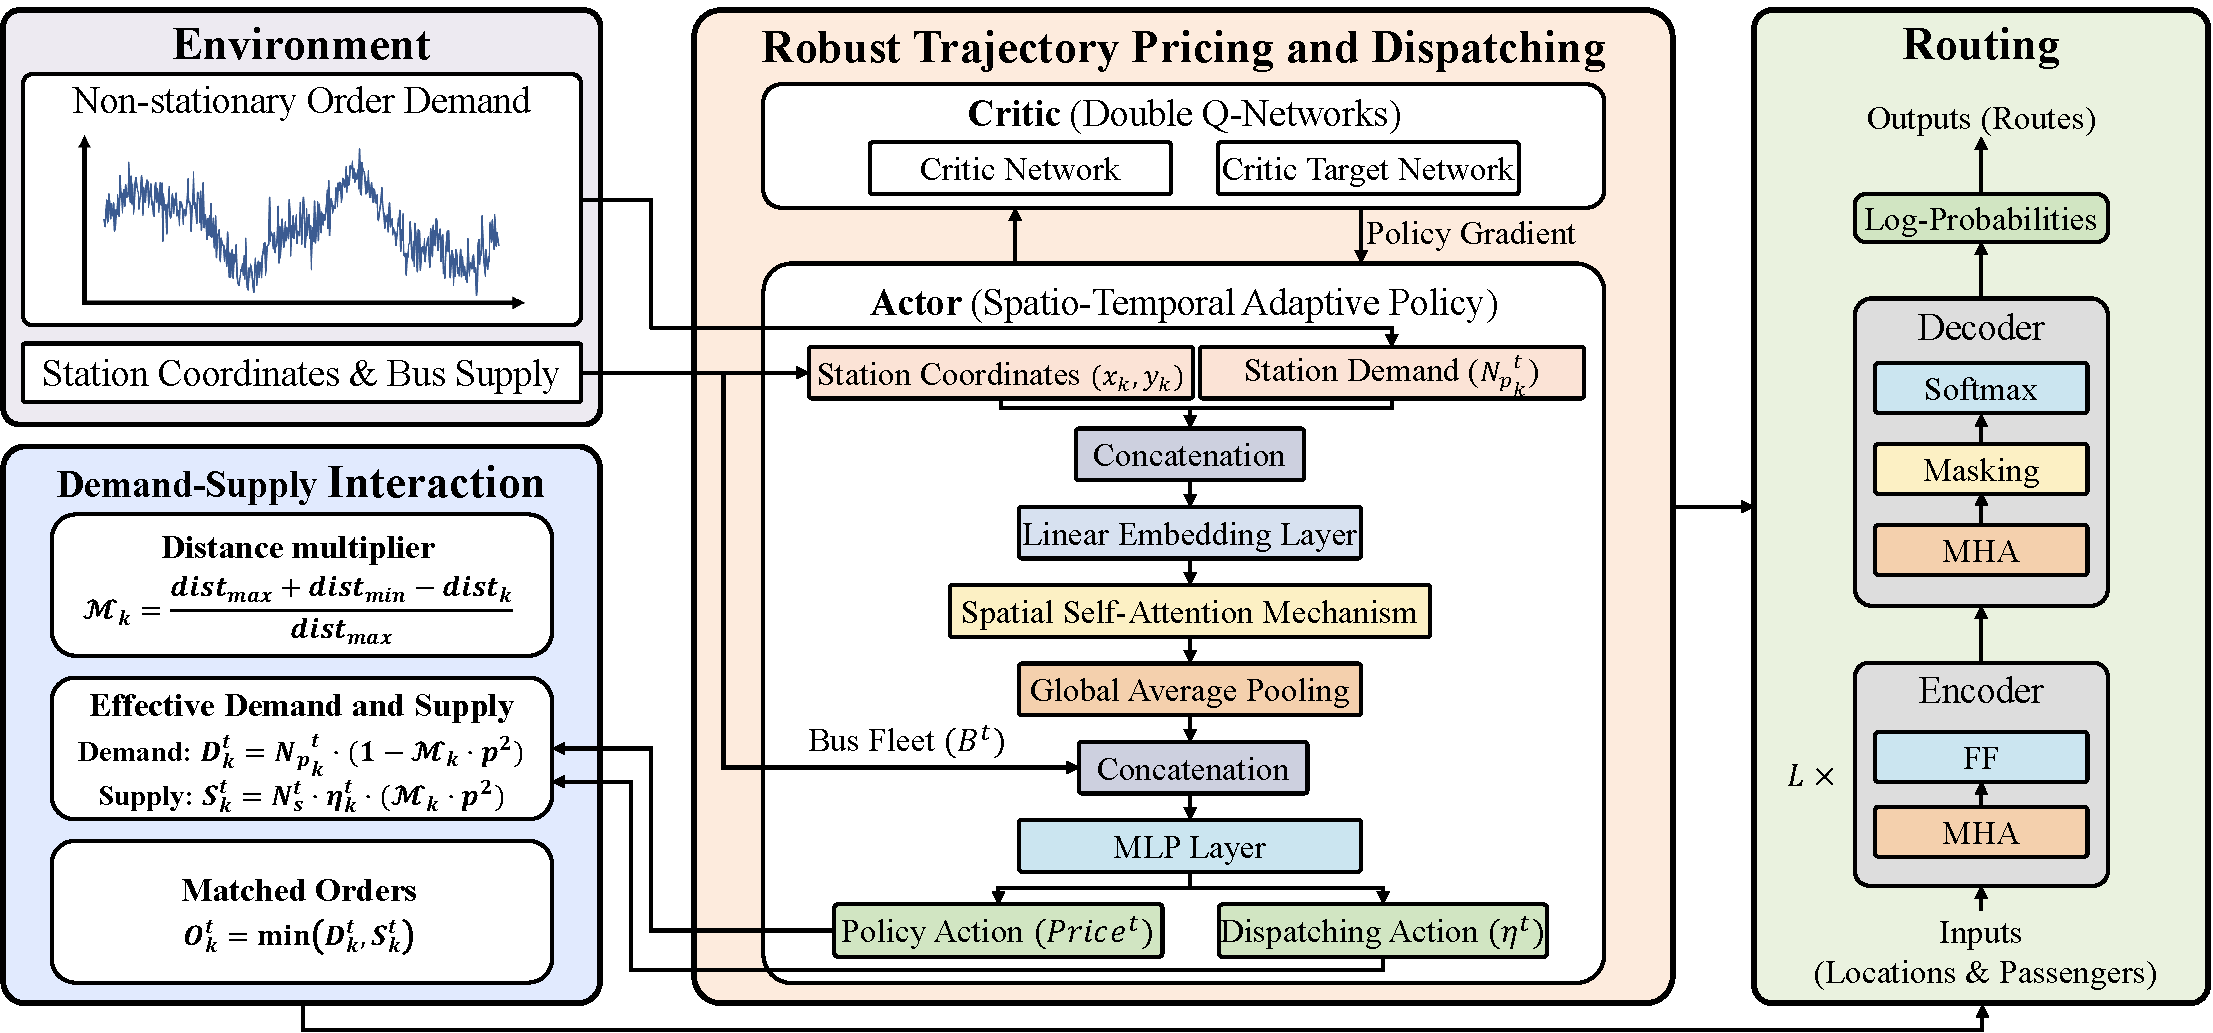
\includegraphics[width=0.9\linewidth]{fig/Framework-journal.pdf}
            \caption{Overview of the ST-SACA method.} 
            \label{fig:framework}
        \end{center}
    \end{boxedminipage}

    \begin{boxedminipage}[htbp]{\linewidth}
        \vspace{2mm}

        The proposed \textbf{ST-SACA} framework is an end-to-end solution designed to address the JDRP problem under dynamic uncertainty. 
        As illustrated in Figure~\ref{fig:framework}, the framework operates in a hierarchical manner: 
        (1) The \textbf{Demand-Supply Interaction} module models how market demand responds to pricing strategies; 
        (2) The \textbf{Robust Trajectory Pricing and Dispatching} module, powered by a Spatio-Temporal Adaptive Actor-Critic agent, determines the optimal pricing and seat allocation to maximize long-term profit; 
        (3) The \textbf{Attention-Based Routing} module utilizes an attention-based network to execute efficient route planning based on the pricing and dispatching decisions.
    \end{boxedminipage}



    \textbf{Distance-aware demand-supply interaction.} Compared with the conference version, the journal manuscript makes the economic mechanism more realistic. Instead of treating destination demand and supply response as homogeneous, the new formulation incorporates the spatial heterogeneity of travel distance into both passenger acceptance and platform supply willingness.

    \begin{tabular}{|p{0.44\textwidth}|p{0.44\textwidth}|}
        \hline
        \textbf{Original Version} & \textbf{New Version}\\
        \hline
        SACA determines the order price and the accepted order set according to the demand and supply relationship through a SAC framework. &
        Considering the spatial heterogeneity, we model the divergent preferences of passengers and the platform regarding travel distance. From the demand side, passengers traveling to farther destinations typically exhibit \textbf{lower price sensitivity} due to the lack of convenient alternatives. Conversely, from the supply side, the platform prefers allocating resources to closer destinations to \textbf{minimize operational costs} and avoid excessive detours.\\
        \hline
    \end{tabular}

    \textbf{Spatio-temporal actor redesign.} We also addressed a key limitation of the conference version: standard reinforcement learning architectures treat spatial states as flat feature vectors and therefore ignore the topological relationships between stations. The journal version replaces this design with a novel \textbf{Spatio-Temporal Adaptive Actor}, which uses coordinate-aware embedding and self-attention to fuse geographical structure with dynamic demand information.
    
    \begin{boxedminipage}[htbp]{\linewidth}
    \vspace{2mm}
    \textbf{Spatio-Temporal Adaptive Actor}
    Standard reinforcement learning approaches often treat the spatial state $\mathbf{N}_p^t$ as a flat feature vector, neglecting the underlying topological dependencies between stations. To enhance robustness, we design a {Spatio-Temporal Adaptive Actor} that explicitly captures the topological dependencies.
    
    \textbf{Spatial Self-Attention Mechanism:} We employ a multi-head self-attention mechanism to model the interactions between stations. The spatially context-aware feature representation $\mathbf{h}_i$ is then updated by aggregating information from the entire network:
    \begin{equation}
        \mathbf{h}_i = \mathbf{e}_i + \sum_{j \in |V|} \alpha_{i,j} (\mathbf{e}_j\mathbf{W}_V).
    \end{equation}
    \end{boxedminipage}

    \textbf{Executable workflow.} We further formalized the operational workflow by presenting pseudo-code for the attention-based route generation, the \textbf{Training Phase}, and the \textbf{Online Execution Procedure}. Instead of only describing the method conceptually, the journal version now specifies how pricing, dispatching, routing, reward calculation, replay-buffer updates, and online deployment interact across the full pipeline.
    
    \begin{tabular}{|p{0.44\textwidth}|p{0.44\textwidth}|}
        \hline
        \textbf{Original Version} & \textbf{New Version}\\
        \hline
        Briefly described per-slot execution and the interaction between SAC and the attention module, but did not formalize the complete training and deployment workflow.
        &
        \textbf{Training Phase:} The framework alternates between interacting with the environment to collect experiences and updating the network parameters. The reward calculation relies on the route distance computed by the routing module.

        \textbf{Online Execution:} Once trained, the model is deployed for real-time decision-making. The pricing and dispatching policy and routing model work sequentially within each time slot to handle the dynamic order batch.\\
        \hline
        \end{tabular}

    \textbf{New theoretical analysis.} We also added a theoretical analysis subsection, which is entirely absent from the conference version. Rather than relying only on empirical evidence, the journal version now provides formal support for both real-time feasibility and robustness under non-stationary demand.
    
    \begin{boxedminipage}[htbp]{\linewidth}
    \vspace{2mm}
    \textbf{Theoretical Analysis}
    In this section, we provide a rigorous analysis of the computational complexity and the theoretical properties concerning the convergence and robustness of the proposed ST-SACA.
    
    \textbf{Computational Complexity Analysis:} The aggregate inference complexity per time slot is $O((|V|^2 + M^2) \cdot d)$. This polynomial complexity ensures that ST-SACA can generate solutions within milliseconds, satisfying the real-time requirements of online bus-booking platforms.
    
    \textbf{Theoretical Robustness:} The robustness of ST-SACA against uncertainty $\lambda^t$ is derived from two key components: \textbf{Lipschitz Continuity of State Representation} and \textbf{Entropy-Regularized Resilience}.
    \end{boxedminipage}

    Overall, Section IV now explains not only \textit{what} decisions are made, but also \textit{how} the framework models realistic passenger-platform interaction, captures spatial dependency, executes online, and remains computationally feasible under non-stationary demand.

    \item[e)] In \textbf{Section V}, we reworked the experimental section from a basic stationary-performance comparison into a robustness-oriented evaluation. The conference version mainly compared SACA with two modular baselines under the historical-data setting. The journal version adds non-stationary demand simulation, stronger robust baselines, ablation studies, efficiency evaluation, parameter sensitivity, and richer case-study visualizations.

    \begin{tabular}{|p{0.44\textwidth}|p{0.44\textwidth}|}
        \hline
        \textbf{Original Version} & \textbf{New Version}\\
        \hline
        The experiments mainly evaluated solution quality on a real-world dataset, compared SACA with DPEA+SubBus and PODP+L2i, and included a sensitivity analysis of $\lambda$ plus a pricing-policy case study. &
        The experiments are reorganized around robustness-oriented research questions: stationary and non-stationary performance, impact of uncertainty degree, ablation of key components, computational efficiency, ORR-weight sensitivity, and qualitative pricing-policy behavior under stronger baselines.\\
        \hline
    \end{tabular}

    \textbf{Uncertainty-aware experimental setup.} We introduced a new \textbf{Experimental Setup} based on a Non-Homogeneous Poisson Process (NHPP), which makes it possible to simulate realistic market volatility and directly test the robust setting defined earlier in the paper.
    
    \begin{boxedminipage}[htbp]{\linewidth}
    \vspace{2mm}
    \textbf{Uncertainty Generation}
    We simulate dynamic market environments by introducing stochastic volatility. We model the order arrival process as a Non-Homogeneous Poisson Process (NHPP). Based on the historical demand baseline $\lambda_{base}$, the time-varying intensity $\lambda(t)$ is modeled as:
    \begin{equation}
        \lambda(t) = \lambda_{base} \cdot (1 + A \sin(\omega t + \varphi))
    \end{equation}
    where $A$ controls the \textbf{Uncertainty Scale} and $\omega$ controls the \textbf{Uncertainty Frequency}. Specifically, a higher $A$ simulates more drastic deviations, while a larger $\omega$ introduces more rapid temporal fluctuations in market conditions, creating a more challenging dynamic environment.
    \end{boxedminipage}

    \textbf{Stronger baselines.} We also expanded the baseline selection into representative two-stage methods, advanced robust/composite methods, and the conference-version SACA as an internal control. This allows the journal version to demonstrate that the gain comes from the new spatio-temporal robust design rather than from weak comparison targets.
    
    \begin{boxedminipage}[htbp]{\linewidth}
    \vspace{2mm}
    \textbf{Baselines}
    Since most existing approaches tackle the problem in a modular fashion, we categorize the baselines based on the architectural complexity and focus on robustness.

    \begin{itemize}
        \item \textbf{Representative Two-Stage Baselines:} These methods represent the standard pipeline paradigm, where pricing/dispatching and routing are solved sequentially using established algorithms.
        \begin{itemize}
            \item \textbf{DPEA+SubBus~\cite{ref:DPEA, ref_shared_subway}:} A standard baseline combining a TRPO algorithm for order pricing and bus scheduling with a heuristic insertion algorithm called SubBus for routing.
            \item \textbf{PODP+L2i~\cite{ref:PODP, ref:L2i}:} A hybrid approach that couples predictive dynamic pricing with \textit{L2i}, a learning-based iterative routing solver.
        \end{itemize}
        
        \item \textbf{Advanced Robust \& Composite Baselines:} These are state-of-the-art (SOTA) methods that employ sophisticated mechanisms to enhance specific performance metrics like fairness or robustness.
        \begin{itemize}
            \item \textbf{GRC-ELG~\cite{ref:Lei2023, ref:Yoon2024IJCAI}:} A composite framework integrating Goal-Conditioned RL with an Ensemble of Local and Global attention mechanism for routing.
            \item \textbf{JDRL-POMO~\cite{ref:Sun2022KDD, ref:KwonPOMO2020}:} A strong baseline for robustness. It combines the JDRL dispatching policy with POMO, a routing solver that uses instance augmentation to enhance routing quality.
        \end{itemize}
    \end{itemize}
    \end{boxedminipage}

    \textbf{Robustness evidence under non-stationary demand.} We broadened the evidence for the journal version by adding non-stationary performance tables and training curves. The new model is compared not only through aggregate metrics, but also through visual evidence of convergence stability.

    \begin{boxedminipage}[htbp]{\linewidth}
    \vspace{2mm}
    \textbf{Performance under Non-Stationary Scenarios}

    \begin{center}
    \captionsetup{font=normalsize}
    \normalsize
    \setlength{\tabcolsep}{5pt}
    \captionof{table}{\textbf{Key results reproduced from Table 5 in the journal manuscript.} Performance under non-stationary scenarios.}
    \begin{tabular}{@{}lcccc@{}}
    \toprule
    Method & Reward & Profit & Cost & ORR \\
    \midrule
    SACA & 21.70 & 21.33 & 12.11 & 0.09 \\
    GRC-ELG & 33.34 & 32.68 & 19.21 & 0.16 \\
    JDRL-POMO & 24.86 & 24.50 & 9.65 & 0.09 \\
    ST-SACA & \textbf{38.70} & \textbf{38.00} & 17.73 & \textbf{0.18} \\
    \bottomrule
    \end{tabular}
    \end{center}

    The reproduced table directly shows that ST-SACA achieves the highest reward and profit under non-stationary demand while also maintaining the highest ORR. Compared with GRC-ELG (\textbf{33.34 / 32.68 / 19.21 / 0.16}) and JDRL-POMO (\textbf{24.86 / 24.50 / 9.65 / 0.09}), the journal version improves economic return and also delivers a more balanced trade-off between service quality and operational cost.

    \textbf{Impact of Uncertainty Degree (RQ2)}

    \begin{center}
    \captionsetup{font=normalsize}
    \normalsize
    \setlength{\tabcolsep}{2.5pt}
    \captionof{table}{\textbf{Key results reproduced from Table 6 in the journal manuscript.} Profit comparison under different uncertainty settings.}
    \begin{tabular}{@{}lcccc@{}}
    \toprule
    Uncertainty Setting & ST-SACA & SACA & GRC-ELG & JDRL-POMO \\
    \midrule
    $A = 1, \omega = 0.5$ & \textbf{30.18} & 22.62 & 29.35 & 27.56 \\
    $A = 1, \omega = 1$ & \textbf{30.23} & 23.32 & 26.31 & 27.27 \\
    $A = 5, \omega = 1$ & \textbf{40.19} & 21.70 & 36.21 & 25.53 \\
    $A = 10, \omega = 1$ & \textbf{38.70} & 20.49 & 33.34 & 24.86 \\
    \bottomrule
    \end{tabular}
    \end{center}

    The reproduced uncertainty table further shows that the advantage of ST-SACA becomes larger as volatility intensifies. Under mild uncertainty ($A = 1, \omega = 0.5$), ST-SACA only improves by about \textbf{+2.8\%} over the strongest baseline GRC-ELG (\textbf{30.18} vs. \textbf{29.35}). Under stronger volatility ($A = 10, \omega = 1$), the gain expands to about \textbf{+16.1\%} (\textbf{38.70} vs. \textbf{33.34}). This quantitative trend complements Figure~\ref{fig:reply_curves}: the journal version is not only more stable during training, but also more robust when the environment becomes increasingly non-stationary.
    \end{boxedminipage}

    \textbf{New Visual Evidence of Robustness.}
    Figure~\ref{fig:reply_curves} is newly added to show the ``Robustness Gap'' more directly. The dashed gray curve corresponds to the conference version (SACA), which oscillates severely under non-stationary demand, whereas the solid red curve corresponds to the journal version (\textbf{ST-SACA}), which converges more steadily and reaches a substantially higher value.

    \begin{boxedminipage}[htbp]{\linewidth}
        \centering
        \makeatletter
        \def\@captype{figure}
        \makeatother

        \captionsetup{font=small}
        \captionsetup[subfloat]{font=scriptsize}

        % \vspace{2mm}
        
        \subfloat[Reward]{
            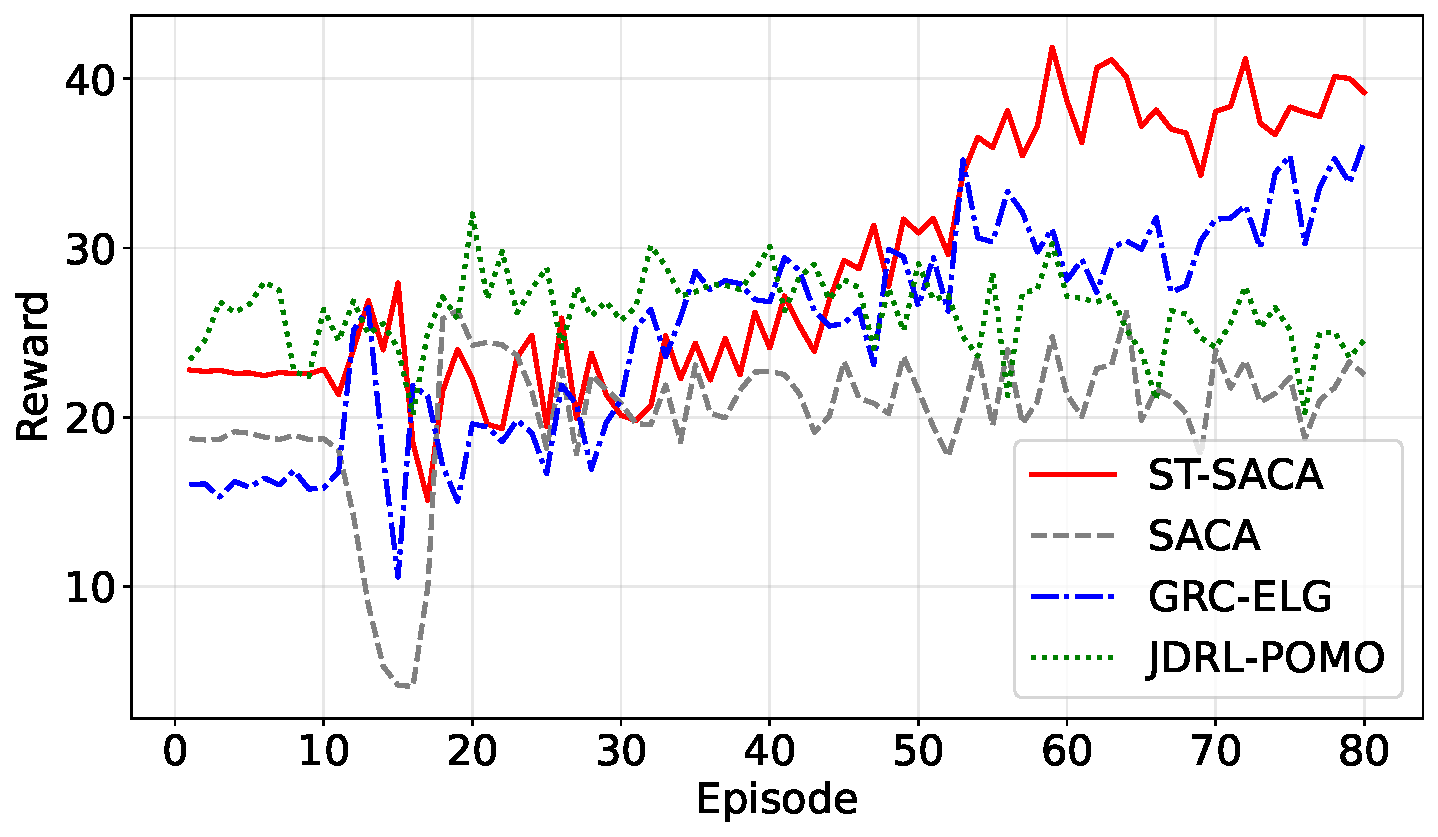
\includegraphics[width=0.48\linewidth]{fig/comparison_total_reward.pdf} 
            \label{fig:reply_curve_reward}
        }
        \hfill
        \subfloat[Profit]{
            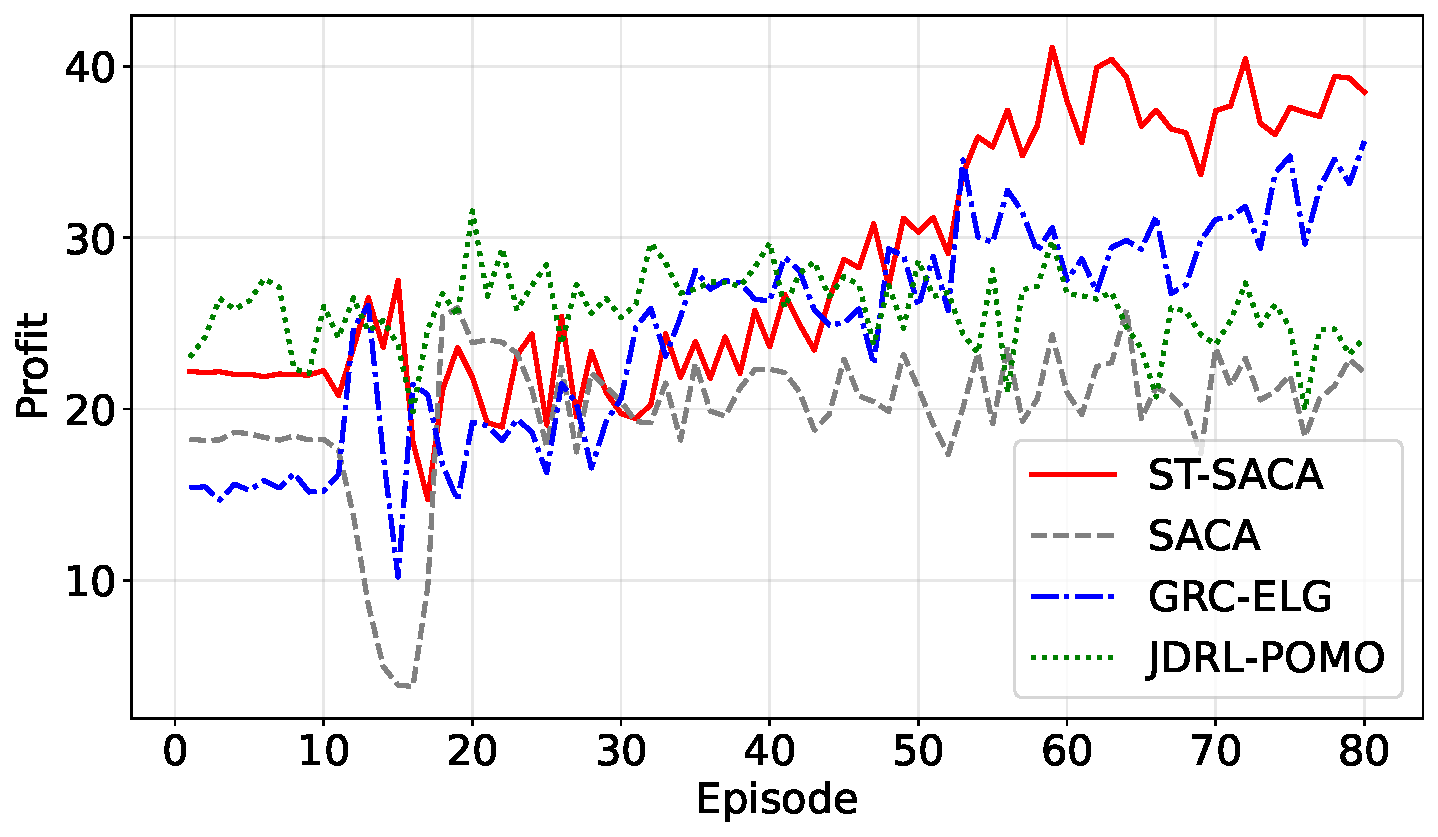
\includegraphics[width=0.48\linewidth]{fig/comparison_revenue.pdf}
            \label{fig:reply_curve_profit}
        }
        \\
        % \vspace{2mm}
        \subfloat[Cost]{
            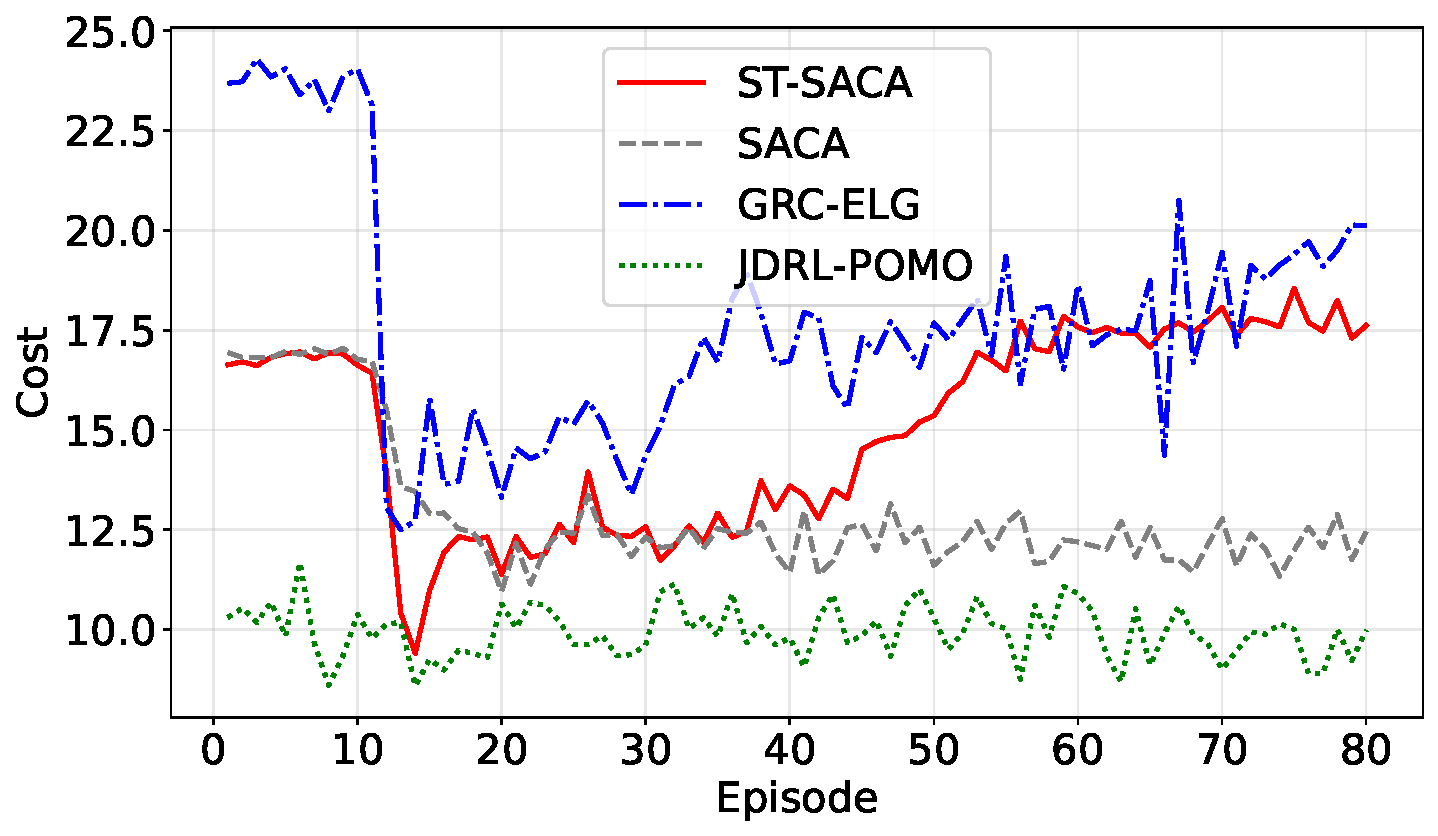
\includegraphics[width=0.48\linewidth]{fig/comparison_cost.pdf}
            \label{fig:reply_curve_cost}
        }
        \hfill
        \subfloat[ORR]{
            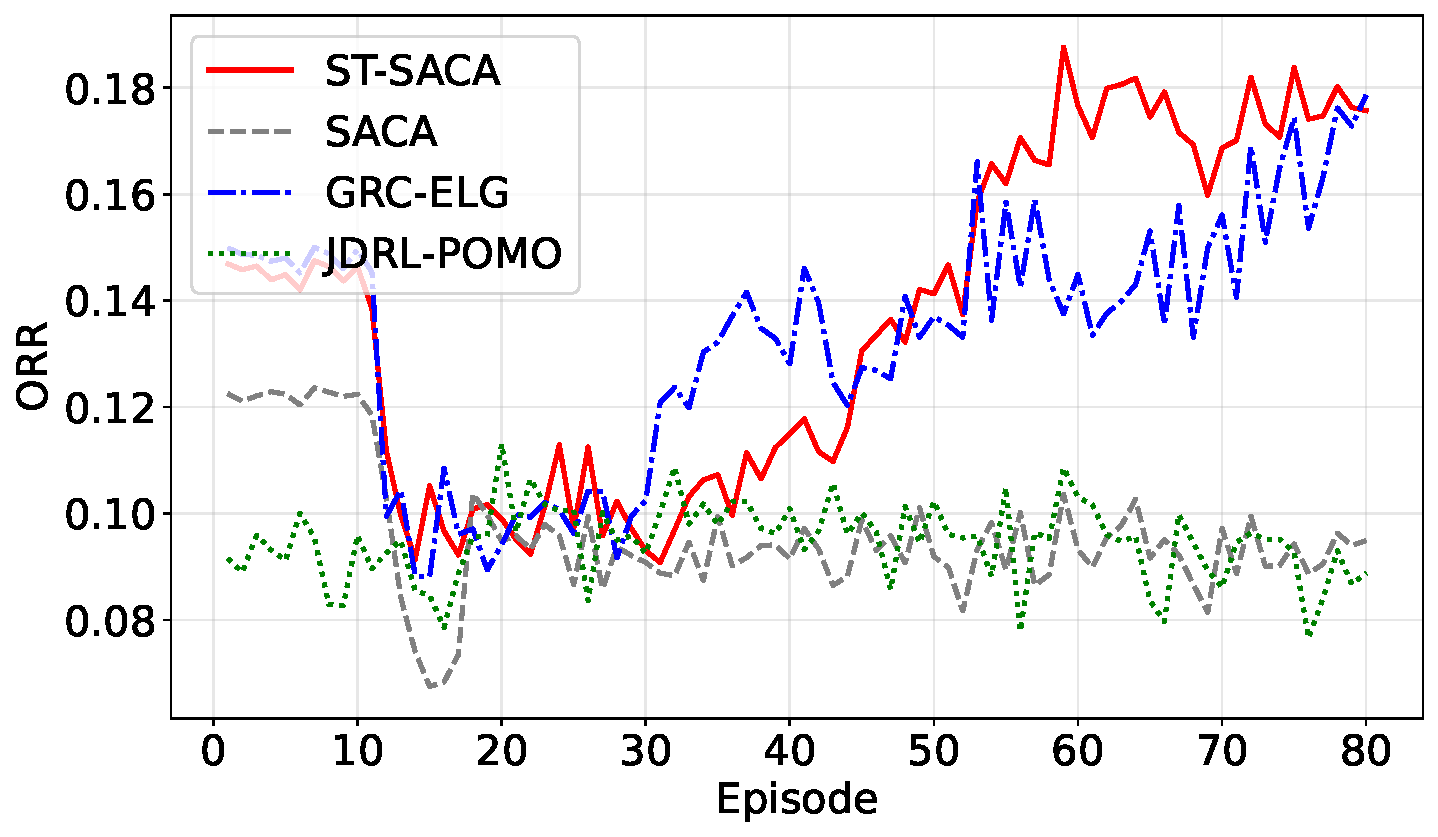
\includegraphics[width=0.48\linewidth]{fig/comparison_orr.pdf}
            \label{fig:reply_curve_orr}
        }
        \captionof{figure}{\textbf{Comparison of training stability.} ST-SACA (red solid line) significantly outperforms the conference version (gray dashed line) and other baselines in non-stationary environments.}
        \label{fig:reply_curves}

        \vspace{2mm}
    \end{boxedminipage}

    \textbf{Component-level and deployment-level validation.} We additionally incorporated a comprehensive \textbf{Ablation Study (RQ3)} and a \textbf{Computational Efficiency (RQ4)} analysis. These experiments show that the journal version improves performance through meaningful architectural changes rather than by introducing impractical computational overhead.
    
    \begin{boxedminipage}[htbp]{\linewidth}
    \vspace{2mm}
    \textbf{Ablation Study (RQ3)}

    \vspace{-6mm}

    \begin{center}
    \captionsetup{font=normalsize}
    \normalsize
    \setlength{\tabcolsep}{2pt}
    \captionof{table}{\textbf{Key results reproduced from Table 7 in the journal manuscript.} Comparison of ST-SACA variants.}
    \begin{tabular}{@{}lccccc@{}}
    \toprule
    Variant & Reward & Profit & Cost & ORR & Dist.(km) \\
    \midrule
    ST-SACA (Full) & \textbf{38.70} & \textbf{38.00} & 17.73 & \textbf{0.18} & 118.23 \\
    w/o Spatial Attn. & 20.49 & 20.12 & 12.03 & 0.09 & 80.22 \\
    w/o Learned Route & 26.98 & 26.62 & 9.71 & 0.09 & 64.73 \\
    w/o ORR Reward & 26.34 & 25.98 & 9.91 & 0.09 & 66.05 \\
    \bottomrule
    \end{tabular}
    \end{center}

    The reproduced ablation table shows that the full ST-SACA achieves the best balance across all metrics. When the Spatio-Temporal Adaptive Actor is removed (\textbf{w/o Spatial Attn.}), the reward drops sharply from \textbf{38.70} to \textbf{20.49} and the ORR is halved from \textbf{0.18} to \textbf{0.09}, which confirms that the journal version's new spatial modeling is essential rather than cosmetic.
    
    \textbf{Impact of the Service-Oriented Reward.} The same reproduced table also shows that removing the ORR reward term (\textbf{w/o ORR Reward}) reduces the reward to \textbf{26.34} and again lowers the ORR to \textbf{0.09}. This result explains why the journal version explicitly introduces a composite reward: without this newly added incentive, the policy degenerates into short-term profit chasing and fails to preserve service coverage.

    \end{boxedminipage}

    \begin{boxedminipage}[htbp]{\linewidth}
    \vspace{2mm}
    
    \textbf{Computational Efficiency (RQ4)}

    \begin{center}
    \captionsetup{font=normalsize}
    \normalsize
    \setlength{\tabcolsep}{7pt}
    \captionof{table}{\textbf{Key results reproduced from Table 8 in the journal manuscript.} Inference time per time slot with varying fleet size.}
    \begin{tabular}{@{}lccccc@{}}
    \toprule
    Bus Num & 10 & 20 & 30 & 40 & 50 \\
    \midrule
    ST-SACA (ms) & 4.7 & 5.9 & 8.6 & 11.9 & 12.5 \\
    \bottomrule
    \end{tabular}
    \end{center}

    The reproduced efficiency table shows that ST-SACA still maintains millisecond-level inference speeds as the fleet size grows, increasing only from \textbf{4.7 ms} for 10 buses to \textbf{12.5 ms} for 50 buses. The journal paper further reports that the full decision process remains around \textbf{45 ms} even with 500 pending orders, which is negligible relative to the 10-minute decision interval. Hence, the additional robustness modules improve performance without undermining online deployability.
    \end{boxedminipage}

    \noindent \textbf{Parameter Sensitivity for Service-Quality Control.}
    We further incorporated Figure~\ref{fig:reply_sensitivity} to explain why the journal version introduces an explicit ORR weight in the composite reward. The journal paper now provides a quantitative analysis of how the reward coefficient $\lambda_{orr}$ controls the balance between profitability and service responsiveness.

    Figure~\ref{fig:reply_sensitivity} shows that \textbf{Average ORR} increases as $\lambda_{orr}$ becomes larger, whereas \textbf{Average Profit} first rises and then declines. This means the journal version does not merely report stronger results, but also explains how the new reward design can be tuned to balance service quality and economic return. This mechanism-level evidence is consistent with Table 6, where ST-SACA maintains only a modest advantage under low uncertainty but expands the gap substantially under severe volatility, and with Table 7, where removing the ORR reward term lowers the ORR from \textbf{0.18} to \textbf{0.09}. Taken together, the added table-based analysis and the new figure make the experimental section much more complete than in the conference version.

    \begin{boxedminipage}[htbp]{\linewidth}
        \centering
        \makeatletter
        \def\@captype{figure}
        \makeatother

        \captionsetup{font=small}
        \vspace{2mm}
        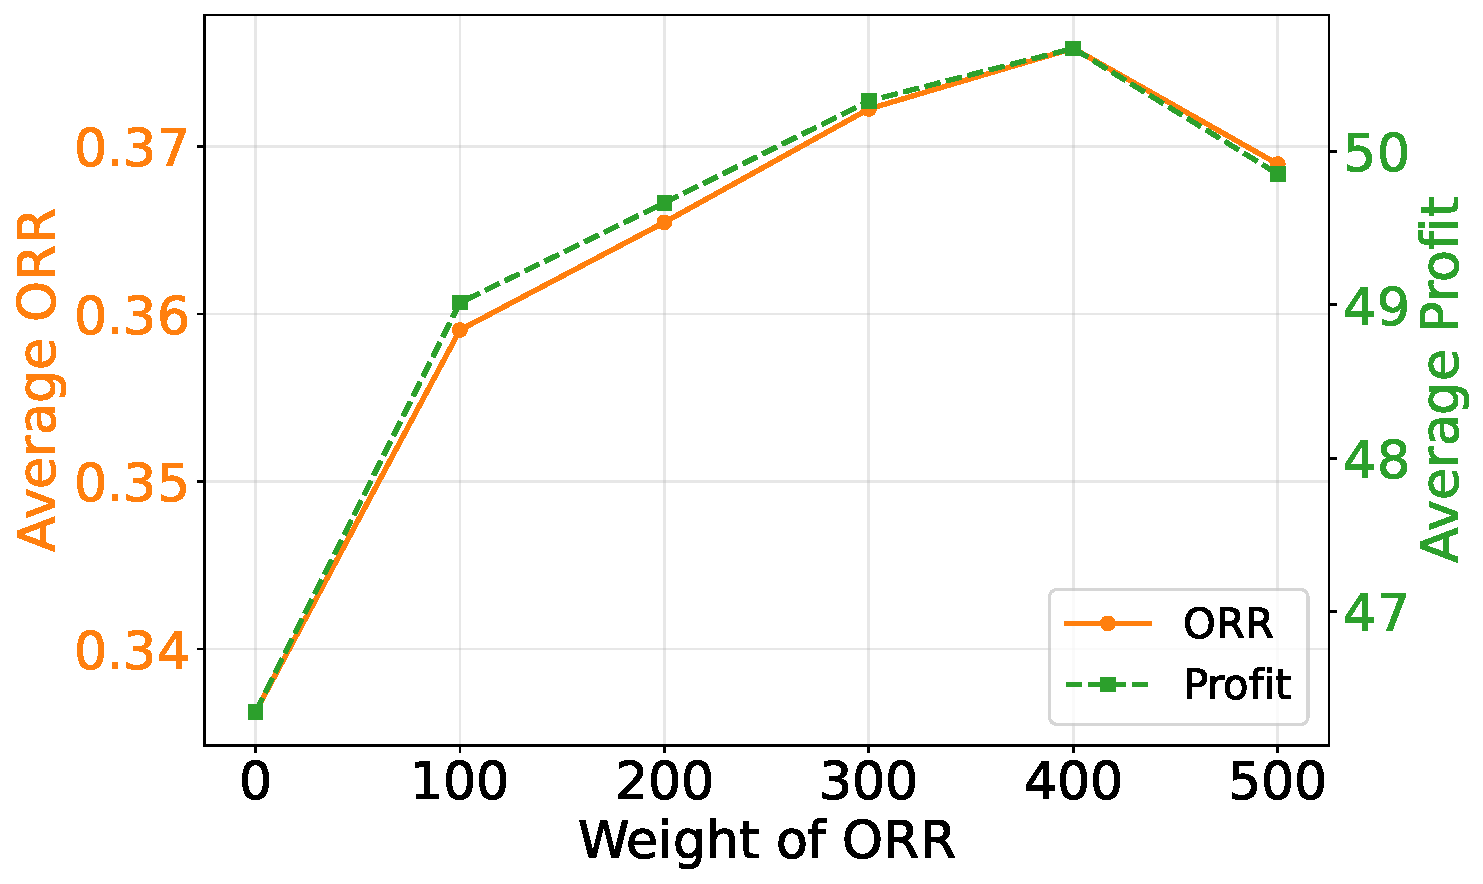
\includegraphics[width=0.6\linewidth]{fig/parameter_sensitivity_orr.pdf}
        \captionof{figure}{\textbf{Sensitivity analysis of the ORR weight.} The journal version further analyzes how the ORR weight affects average profit and average ORR.}
        \label{fig:reply_sensitivity}
        \vspace{2mm}
    \end{boxedminipage}

\noindent \textbf{Mechanism-Oriented Case Study Visualization:}
We also enriched the case study with Figure~\ref{fig:reply_heatmaps}, which compares the pricing heatmaps of the conference and journal versions together with robust baselines.
\begin{itemize}
    \item \textbf{Figure \ref{fig:reply_pot}} shows the ground-truth potential demand, where station (5,5) is a clear hotspot (dark red).
    \item \textbf{Figure \ref{fig:reply_st_saca}} shows that our new \textbf{ST-SACA} intelligently sets a significantly higher price for this hotspot to maximize revenue.
    \item \textbf{Figure \ref{fig:reply_saca}} shows that the conference model (\textbf{SACA}) fails to capture this opportunity, setting a mediocre price (lighter color).
\end{itemize}
This newly added visual comparison shows that the distance-aware demand-supply function in the journal version enables the agent to learn more granular and profitable pricing strategies. By assigning higher prices to demand hotspots while setting prohibitive prices for distant, low-margin regions, ST-SACA avoids inefficient long-distance detours and reveals a stronger link between pricing decisions and routing efficiency than was shown in the conference paper.

    \begin{boxedminipage}[htbp]{\linewidth}
        \centering
        \makeatletter
        \def\@captype{figure}
        \makeatother
        
        \captionsetup{font=small}
        \captionsetup[subfloat]{font=scriptsize}
        
        \subfloat[Potential demand]{
            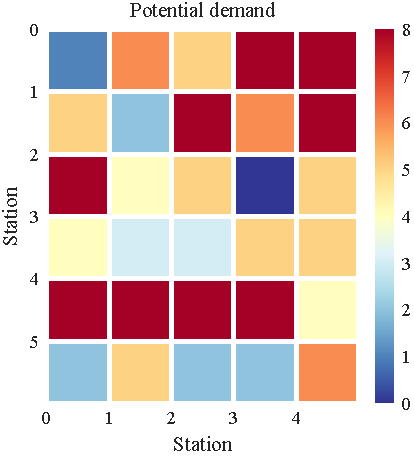
\includegraphics[width=0.31\linewidth]{fig/case_study_pricing_demand.pdf}
            \label{fig:reply_pot}
        }
        \hfill
        \subfloat[Pricing of \textbf{ST-SACA} (New)]{
            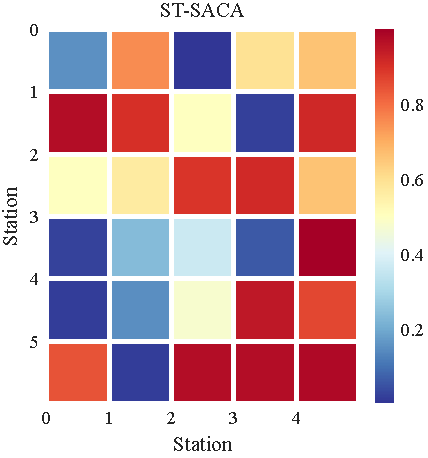
\includegraphics[width=0.31\linewidth]{fig/case_study_pricing_st_saca.pdf}
            \label{fig:reply_st_saca}
        }
        \hfill
        \subfloat[Pricing of SACA (Old)]{
            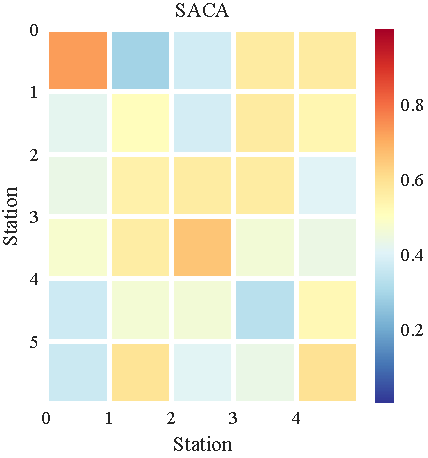
\includegraphics[width=0.31\linewidth]{fig/case_study_pricing_saca.pdf}
            \label{fig:reply_saca}
        }
        
        \vspace{2mm}
        
        \subfloat[Pricing of JDRL-POMO]{
            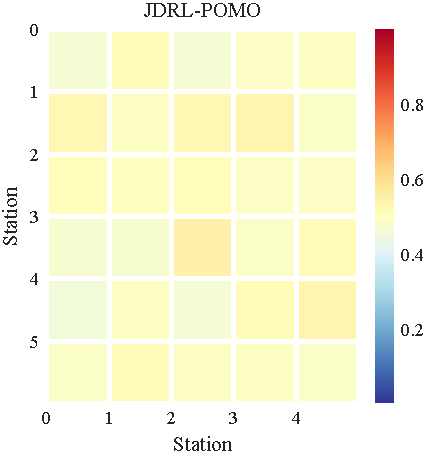
\includegraphics[width=0.31\linewidth]{fig/case_study_pricing_jdrl_pomo.pdf}
            \label{fig:reply_jdrl}
        }
        \hspace{4mm} 
        \subfloat[Pricing of GRC-ELG]{
            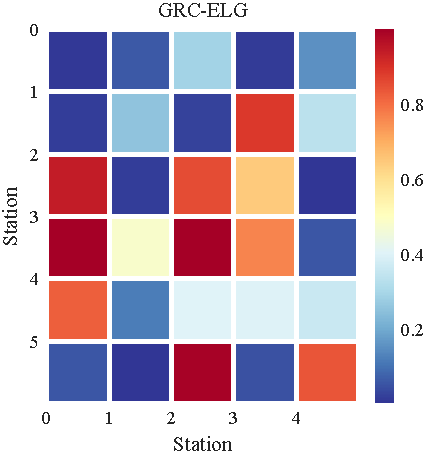
\includegraphics[width=0.31\linewidth]{fig/case_study_pricing_grc_elg.pdf}
            \label{fig:reply_grc}
        }
        
        \captionof{figure}{\textbf{Visual comparison of pricing strategies.} ST-SACA accurately identifies high-demand regions and adjusts prices accordingly, whereas the conference version SACA and other baselines fail to fully exploit these opportunities.}
        \label{fig:reply_heatmaps}
    \end{boxedminipage}

\noindent Overall, Section V now provides a much stronger validation package. The conference version mainly showed that reinforcement learning could improve revenue in a stationary setting, whereas the journal version verifies profitability, robustness, service quality, component necessity, computational feasibility, and policy interpretability under more realistic conditions.


\end{itemize}

\newpage
% \balance
%----------Bibliography---------

\bibliographystyle{IEEEtran}

\bibliography{ref}

\end{document}
